%%%%%%%%%%%%%%%%%%%%%%%%%%%%%%%%%%%%%%%%%
% Beamer Presentation
% LaTeX Template
% Version 1.0 (10/11/12)
%
% This template has been downloaded from:
% http://www.LaTeXTemplates.com
%
% License:
% CC BY-NC-SA 3.0 (http://creativecommons.org/licenses/by-nc-sa/3.0/)
%
%%%%%%%%%%%%%%%%%%%%%%%%%%%%%%%%%%%%%%%%%

%----------------------------------------------------------------------------------------
%	PACKAGES AND THEMES
%----------------------------------------------------------------------------------------

\documentclass{beamer}

\mode<presentation> {

% The Beamer class comes with a number of default slide themes
% which change the colors and layouts of slides. Below this is a list
% of all the themes, uncomment each in turn to see what they look like.

%\usetheme{default}
%\usetheme{AnnArbor}
%\usetheme{Antibes}
%\usetheme{Bergen}
%\usetheme{Berkeley}
%\usetheme{Berlin}
%\usetheme{Boadilla}
%\usetheme{CambridgeUS}
%\usetheme{Copenhagen}
%\usetheme{Darmstadt}
%\usetheme{Dresden}
%\usetheme{Frankfurt}
%\usetheme{Goettingen}
%\usetheme{Hannover}
%\usetheme{Ilmenau}
%\usetheme{JuanLesPins}
%\usetheme{Luebeck}
\usetheme{Madrid}
%\usetheme{Malmoe}
%\usetheme{Marburg}
%\usetheme{Montpellier}
%\usetheme{PaloAlto}
%\usetheme{Pittsburgh}
%\usetheme{Rochester}
%\usetheme{Singapore}
%\usetheme{Szeged}
%\usetheme{Warsaw}

% As well as themes, the Beamer class has a number of color themes
% for any slide theme. Uncomment each of these in turn to see how it
% changes the colors of your current slide theme.

%\usecolortheme{albatross}
%\usecolortheme{beaver}
%\usecolortheme{beetle}
%\usecolortheme{crane}
%\usecolortheme{dolphin}
%\usecolortheme{dove}
%\usecolortheme{fly}
%\usecolortheme{lily}
%\usecolortheme{orchid}
%\usecolortheme{rose}
%\usecolortheme{seagull}
%\usecolortheme{seahorse}
%\usecolortheme{whale}
%\usecolortheme{wolverine}

%\setbeamertemplate{footline} % To remove the footer line in all slides uncomment this line
%\setbeamertemplate{footline}[page number] % To replace the footer line in all slides with a simple slide count uncomment this line

%\setbeamertemplate{navigation symbols}{} % To remove the navigation symbols from the bottom of all slides uncomment this line
}

\usepackage{graphicx} % Allows including images
\usepackage{booktabs} % Allows the use of \toprule, \midrule and \bottomrule in tables
\usepackage{listings}
\usepackage{amsmath}
\usepackage{algpseudocode,algorithm,algorithmicx}

\lstdefinestyle{customjava}{
  breaklines=true,
  frame=L,
  xleftmargin=\parindent,
  language=Java,
  showstringspaces=false,
  basicstyle=\footnotesize\ttfamily,
  keywordstyle=\bfseries\color{green!40!black},
  commentstyle=\itshape\color{gray!40!black},
  identifierstyle=\color{blue},
  stringstyle=\color{orange},
}

%----------------------------------------------------------------------------------------
%	TITLE PAGE
%----------------------------------------------------------------------------------------

\title[Reliable Data Delivery]{Reliable Data Delivery} % The short title appears at the bottom of every slide, the full title is only on the title page

\author{Jonathan Windle} % Your name
\institute[UEA] % Your institution as it will appear on the bottom of every slide, may be shorthand to save space
{
University of East Anglia \\ % Your institution for the title page
\medskip
\textit{J.Windle@uea.ac.uk} % Your email address
}
\date{\today} % Date, can be changed to a custom date

\begin{document}

\begin{frame}
\titlepage % Print the title page as the first slide
\end{frame}

\begin{frame}[allowframebreaks]
\frametitle{Overview} % Table of contents slide, comment this block out to remove it
\tableofcontents % Throughout your presentation, if you choose to use \section{} and \subsection{} commands, these will automatically be printed on this slide as an overview of your presentation
\end{frame}

%-----------------------------------------------------------------
\section{Intro}
\begin{frame}
\frametitle{Intro}
\begin{itemize}
\item Errors in underlying network (lower layers) introduce errors that ultimately lead to packet loss.
\item Transport layer should hide these errors from upper layers.
\item Transport layer solutions:
\begin{itemize}
\item Stop and Wait (or Idle RQ) protocol to provide an inefficient error-free stream of messages.
\end{itemize}
\end{itemize}
\end{frame}
%----------------------------------------------------------------
\section{Terminology}
\begin{frame}
\frametitle{Terminology}
\begin{itemize}
\item \textbf{Data rate:} Is a measure of the speed of data transmission. It is measured in bits per second.
\item \textbf{Error rate:} Is an estimte of the reliability of a communication channel. It is the proportion of corrupted bits to uncorrupted bits.\\
e.g. Domestic telephone lines have an error rate of 1 : 100 000.
\end{itemize}
\end{frame}
%------------------------------------------------------------------
\section{Transport Protocol Data Unit}
\begin{frame}
\frametitle{Transport Protocol Data Unit (TPDU)}
\begin{itemize}
\item Messages sent from transport entity to transport entity are sent in TPDU's (e.g. using TCP or UDP Layer 4 protocols).
\item TPDU's comprise header and application message:
\item Header:
\begin{itemize}
\item Source and destination process IDs.
\item Identifier to indicate TPDU contains information (00).
\item Message length indicator.
\end{itemize}
\item Application message:
\begin{itemize}
\item Payload comprises packet from layer above.
\end{itemize}
\item Errors can occur in either header or message at any section of the TPDU.
\end{itemize}

\includegraphics[scale=0.3]{tpdu.png}
\end{frame}
%-----------------------------------------------------------------
\section{Consequence of Errors}
\begin{frame}
\frametitle{Consequence of Errors}
\begin{itemize}
\item \textbf{Destination process ID:} TPDU is not delivered to the receiver.
\item \textbf{Source Process ID:} Reply is not returned to the original sender.
\item \textbf{Transport layer payload:} Requires an error detectoin mechanism.
\item \textbf{Length field/End of mesaage:} Only part of the TPDU is received.
\item Acknowledgement Schemes:
\begin{itemize}
\item Positive-Only Acknowledgement Scheme: ACK's. (Stop - Wait protocol).
\item Full Acknowledgement Scheme: ACK's and NAK's (Negative Acknowledgement).
\end{itemize}
\end{itemize}
\end{frame}
%------------------------------------------------------------------
\section{Stop and Wait protocol}
\begin{frame}
\frametitle{Stop and Wait protocol}
\begin{columns}[c]
\column{.6\textwidth}
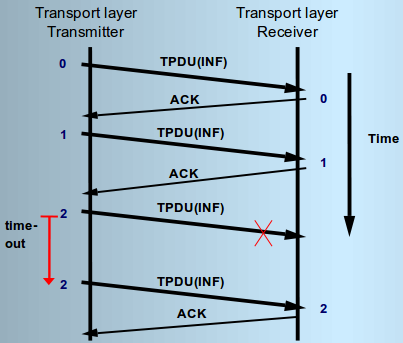
\includegraphics[scale=0.55]{sw.png}
\column{.35\textwidth}
\begin{itemize}
\item Receiver sends an ACK in response to a correctly received TPDU.
\item Transmitter starts a timer when it sends the TPDU.
\item If this times out:
\begin{enumerate}
\item Enquired receiver of the nature of the problem, or:
\item Simply retransmits the TPDU.
\end{enumerate}
\end{itemize}
\end{columns}
\end{frame}
%----------------------------------------------------------------
\subsection{Some notes}
\begin{frame}
\frametitle{Some notes}
\begin{itemize}
\item Positive-only scheme can handle destination address corruption (assuming an incorrect destination does not respond).
\item Timers and time-outs are still needed tocope with errors in source and destination addresses- no ACK or NAK will be received at sender.
\item On timing out, immediate retransmition of TPDU can be more efficient but requires a limit to number of re-tries - in case receiver has crashed.
\item Still inadequate as ACKs and NAKs are themselves (short) TPDUs prone to corruption.
\item If these are lost or corrupter the receiver cannot know if it is receiving a retransmitted last TPDU or the next TPDU.
\item Solution is for TPDUs to contain a sequence number - receiver can detect multiple TPDUs.
\begin{itemize}
\item Use one bit to reduce overhead and switch 0-1-0-1-0 etc. and if 0-0 is received then it is a duplicate.
\end{itemize}
\end{itemize}
\end{frame}
%-----------------------------------------------------------------
\subsection{Example With Numbering}
\begin{frame}
\frametitle{Example With Numbering}
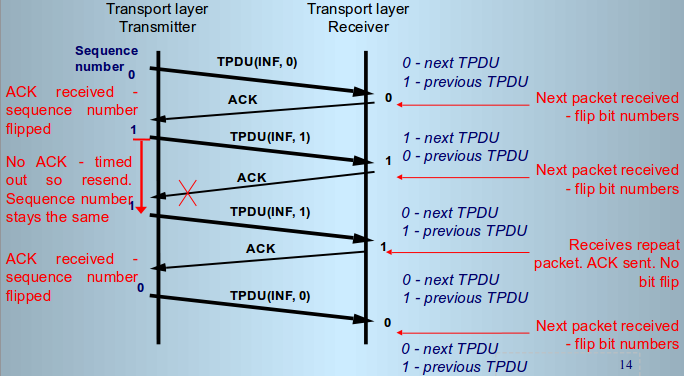
\includegraphics[scale=0.5]{swn.png}
\end{frame}
%----------------------------------------------------------------
\subsection{Review}
\begin{frame}
\frametitle{Review}
\begin{itemize}
\item Transport layer needs fields for:
\begin{itemize}
\item Source and destination IDs
\item Length field or end of TPDU indicator.
\item Sequence number and the payload itself.
\end{itemize}
\item Need for an acknowledgement scheme.
\item Need for timer and timeouts and limited retries at the transmitter.
\item Use of the TPDU sequence number to allow the receiver to detect duplicate TPDUs.
\item Receiver sends packet and then stops and waits until acknowledgement of arrival comes through, or times-out.
\item Issue is that the transmitter cannot proceed to transmit the next message until it receives an ACK / times-out.
\item Solution is to use sliding window protocols
\end{itemize}
\end{frame}
%------------------------------------------------------------------
\section{Sliding Window Protocols}
\begin{frame}
\frametitle{Sliding Window Protocols}
\begin{itemize}
\item Need for more efficient Connection Orientated Protocols.
\item Problem is the transmitter waits for an ACK after each message
\item Solution is to remove the restriction and allow the transmitter too have N messages in transit whose ACK have not been recived yet.
\item This is the basis of sliding window protocols.
\item Stop wait is a special case of sliding window where window size is 1.
\item Also known as {\color{red}pipeline protocols}.
\item Two types:
\begin{itemize}
\item Go Back N
\item Selective Repeat
\end{itemize}
\end{itemize}
\end{frame}
%----------------------------------------------------------------
\subsection{Go back N}
\begin{frame}
\frametitle{Go back N}
\begin{itemize}
\item Transmitter is said to have a Send Window of size N.
\item Requirements are:
\begin{itemize}
\item Buffering at Transmitter:
\begin{itemize}
\item Buffer N messages.
\end{itemize}
\item Sequence Numbers:
\begin{itemize}
\item Sequence numbers can be 0 to Num. SeqNos - 1.
\end{itemize}
\item The Send Window:
\begin{itemize}
\item Range of consecutive Num SeqNs - 1 values.
\end{itemize}
\item The Receive Window:
\begin{itemize}
\item Tracks sequence number of the next message it expects and discards all other messages.
\end{itemize}
\item Acknowledgements:
\begin{itemize}
\item On receipt of ACK, the sender can advance its send window to be the set of values ranging from ACK to (ACK+SeqNo-2)\%SeqNo.
\end{itemize}
\item On Error:
\begin{itemize}
\item The receiver either sends a NAK, or the transmitter times out.
\item The transmitter re-transmits the message and all subsequent messages. Hence Go-Back-N.
\end{itemize}
\end{itemize}
\end{itemize}
\end{frame}
%-----------------------------------------------------------------
\subsubsection{Example}
\begin{frame}
\frametitle{Example}
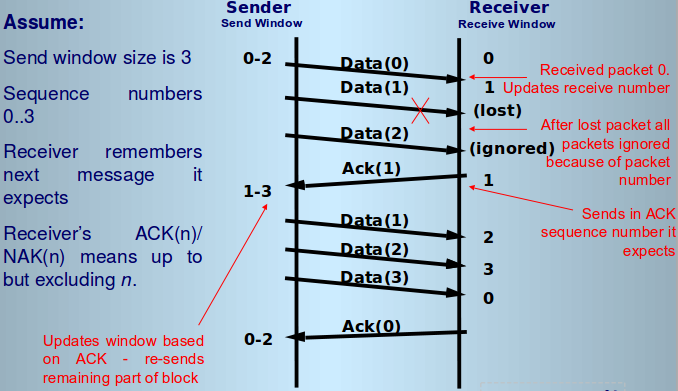
\includegraphics[scale=0.5]{nex.png}
\end{frame}
%---------------------------------------------------------------
\section{Selective Repeat}
\begin{frame}
\frametitle{Selective Repeat}
\begin{itemize}
\item Rather than transmitting block of frames following first lost packet (as with Go Back N), better method is to simply retransmit only those packets which were lost (or in error).
\item This is selective Repeat protocol.
\item Must be able to receive packets out of sequence and be able to buffer these until the sequence can be restored - following repeated re-transmission.
\item Receiver must have a Receive Window of X messages.
\end{itemize}
\end{frame}
%------------------------------------------------------------------
\subsection{Example}
\begin{frame}
\frametitle{Example}
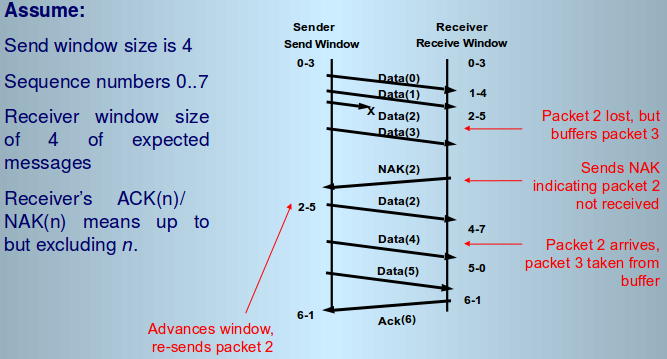
\includegraphics[scale=0.5]{srep.png}
\end{frame}
%----------------------------------------------------------------
\section{Summary}
\begin{frame}
\frametitle{Summary}
\begin{itemize}
\item Simple Stop-Wait protocol is inefficient.
\item Sliding Window (pipeline) protocols allow:
\begin{itemize}
\item Transmitter to transmit sequences of messages.
\item Remove the delay waiting for individual ACKs.
\end{itemize}
\item Go-Back-N is a simple technique which requires minimum resources at the receiver but involves sme unnecessary re-transmissions.
\item Selective Repeat avoids unnecessary re-transmissions but requires additional buffering at the receiver.
\item Both need additional buffering, multiple timers.
\end{itemize}
\end{frame}
%-----------------------------------------------------------------
\begin{frame} 
\Huge{\centerline{The End}}
\end{frame}
\end{document}